\documentclass[12pt]{article}

% import packages
\usepackage[utf8]{inputenc}
\usepackage{float}
\usepackage{subfloat}
\usepackage{subfig}
\usepackage[fleqn]{amsmath}
\usepackage[toc,page]{appendix}
\usepackage{caption}
\usepackage{graphicx}
\usepackage{hyperref}
\usepackage{amssymb}
\usepackage[left=1in,top=0.75in,right=1in,bottom=0.75in]{geometry}

\graphicspath{ {./images} }
% hyperref setup
\hypersetup{
	colorlinks=true,
	linkcolor=blue,
	filecolor=blue,      
	urlcolor=blue,
	citecolor=blue,
	pdftitle={Structural design lab report},
	pdfpagemode=FullScreen,
}
% titlepage	
\title{\textbf{Structural design lab report}}
\author{Callum Stephenson, css47}
\date{1st May 2022}
\begin{document}
    \begin{titlepage}
        \maketitle
        \thispagestyle{empty}
        \vspace{13cm}
        \textbf{Department of Engineering, University of Cambridge}
    \end{titlepage}
    \newpage
    \tableofcontents
    \newpage
    \section{Summary}
        Within this report the aim was to design a cantilever which was able to withstand 1.35 kN and fail within $\pm$5\% of double the load - dubbed the "ultimate load". 
        The structure chosen was a right angle design - which was calculated to fail in buckling due to the stresses around the ultimate load being enough to cause mode A buckling
        of the compression strut. During testing, this was indeed the failure mechanism which occured - this is as the rest of the failure mechanisms were calculated to happen at a lot
        higher stresses than those at ultimate load. Overengineering certain aspects caused a greater weight than necessary, but allowed ease in calculation and ensured that 
        different methods of failure did not interact with one another. 
    \section{Introduction}
        The aim of this report is to show the design process for the end-loaded cantilever problem. The details of this problem are as follows:
        the cantilever was to be 815mm long, withstand load of 1.35 kN and fail within $\pm$5\% of double the load. The goal is to make the cheapest
        cost structure that is able to fulfil these requirements, such as not to overengineer the structure. The allowed materials included plate aluminium,
        aluminium angle, rivets and standard bolts. The following report aims to direct the reader through the process until finality, with testing results
        and explanation of actual failure mode with comparison to expected failure mode.
    \section{Design process}
        \subsection{Starting designs}
                At first, a simple right angle cantilever was drawn with a straight bottom member and the forces in each bar (assuming $\frac{W}{2}$ on each side of the structure in 3D)
                to understand the tension force which the top member would have to carry. Self weight was ignored due to how low the forces were in comparison to load. $T_1$ and $T_2$
                are the forces in the tension and compression member respectively.
                \begin{align}
                    T_1 \sin \theta &= 1350 \\
                    \nonumber \therefore T_1 &= 4520 N \\
                    \nonumber T_2 &= T_1 \cos \theta \\
                    \nonumber \therefore T_2 &= 4310 N
                \end{align}
                An isoscles design was considered, but abandoned due to the uncertainty of length meaning manufacturing defects would have a bigger impact on the design's performance
                due to buckling failure if one member was longer than the other. For this reason, it was decided to progress the right angle design further and begin implementing measures
                which would prevent buckling and allow the rivets to withstand the shear forces. Pictured below are the two reduced 2D designs.
                \begin{figure}[H]
                    \begin{center}
                    \captionsetup{labelfont=bf}
                    \captionsetup{justification=centering}
                    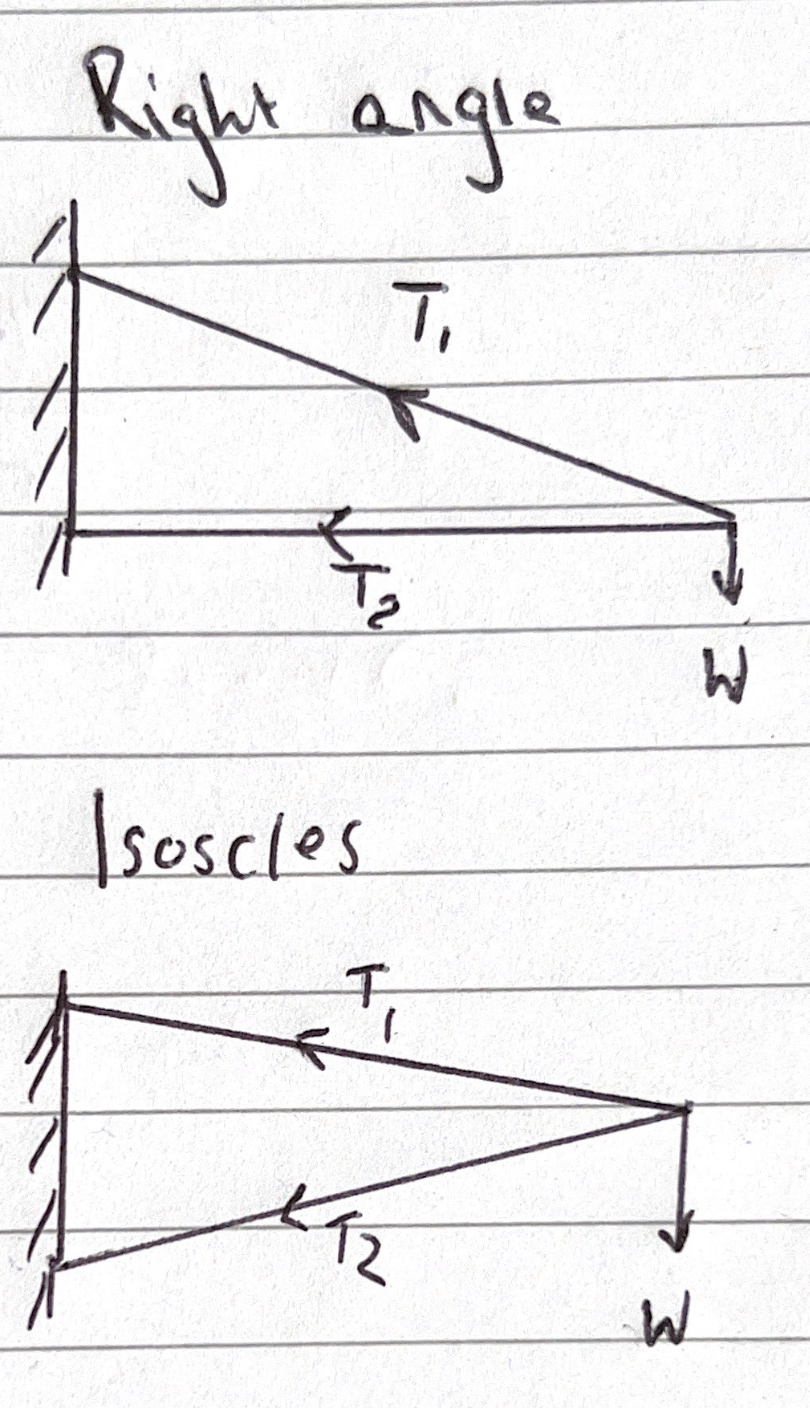
\includegraphics[height=13pc]{init_design.png}
                    \caption{Figure showing the 2D right angle and isoscles cantilevers}
                    \end{center}
                \end{figure}
            \subsection{Calculations to finalise design}
                Calculations were employed in order to bring the design from the simple right angle truss to a final design by accounting for phenomena such as buckling and considering
                the force that each rivet and bolt would need to withstand, as well as considering how to avoid reduction by having too many rivets too close.
                \subsubsection{Buckling}
                    The aim in the buckling calculations is to reduce the biggest unsupported length to one such that when the ultimate load is reached, it would just about buckle.
                    The biggest unsupported member in compression is the bottom compression member of length 815 mm. The maximum load on each side is 1.35 kN - so that is when it would
                    be preferable to have the beam buckle. Easiest way to split the 815 mm is to half it and do calculations based on 407.5 mm. The L/b for the 19.5 x 19.5 x 2 mm
                    is 20.9 - this has been marked on the graph below. 19.5mm was chosen for the 4 main members as it removed the need to calculate rivet spacing for members joined in T arrangement.
                    \begin{figure}[H]
                        \begin{center}
                        \captionsetup{labelfont=bf}
                        \captionsetup{justification=centering}
                        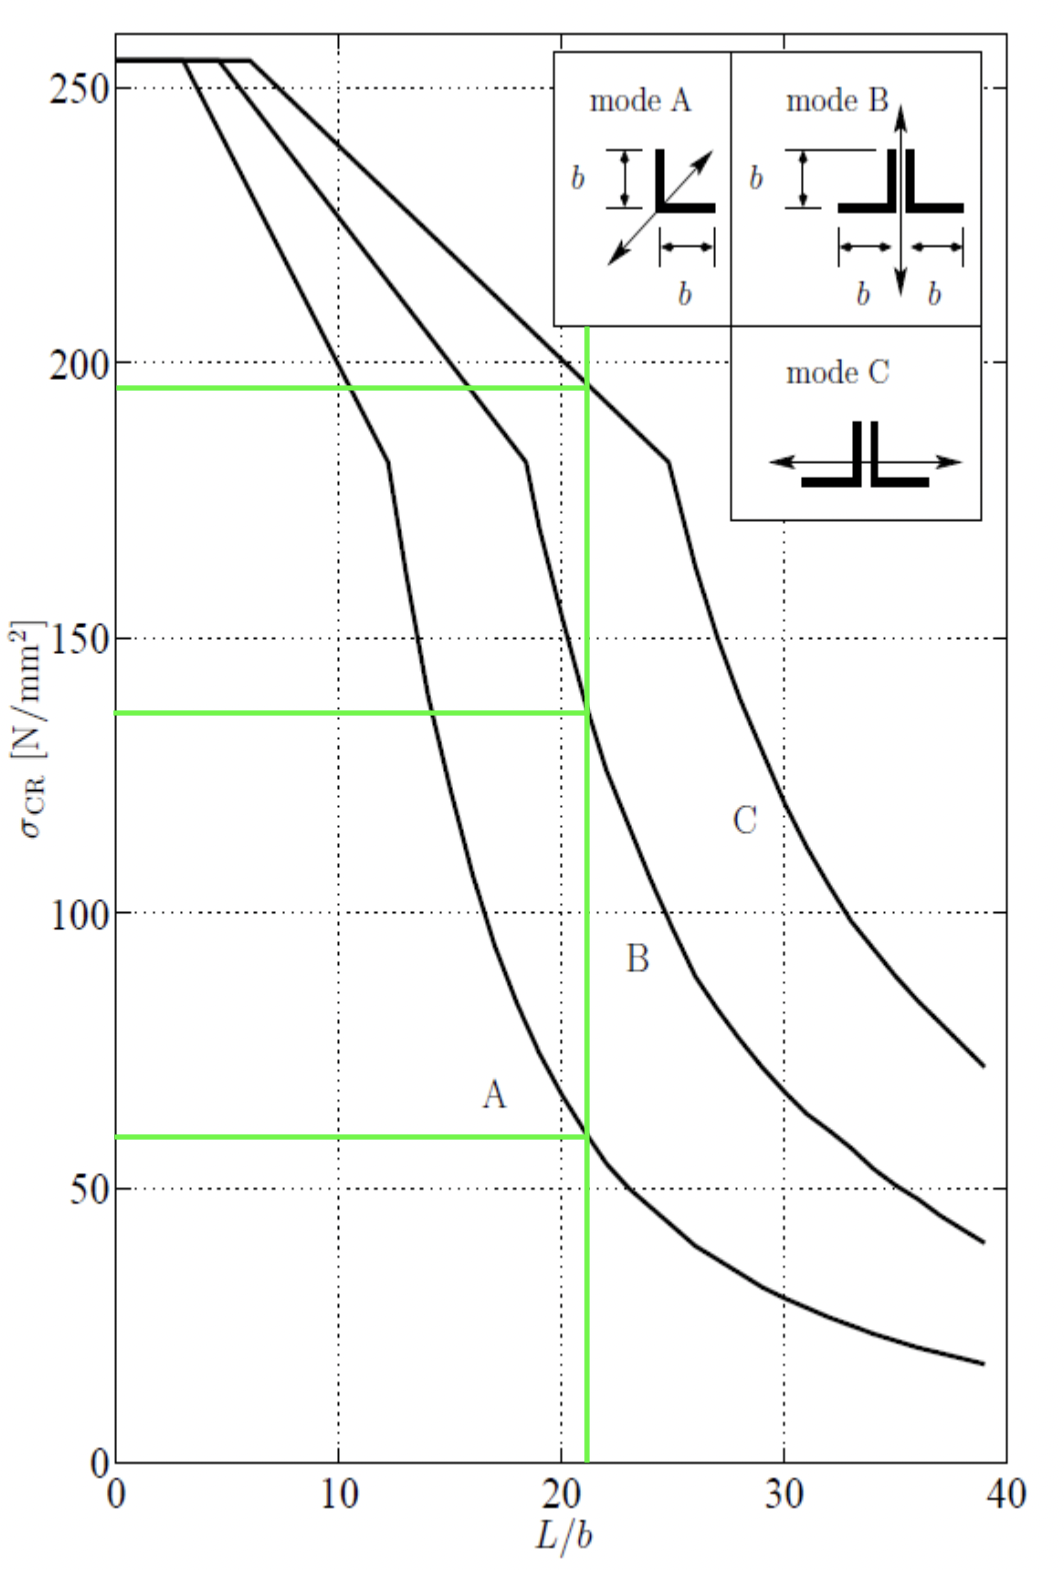
\includegraphics[height=30pc]{buckling.png}
                        \caption{Figure showing buckling values in mode A,B,C for Al 6082-T6}
                        \end{center}
                    \end{figure}
                    It can be seen that the maximum stress in mode A is around 60 N / mm$^2$.
                    \begin{figure}[H]
                        \begin{center}
                        \captionsetup{labelfont=bf}
                        \captionsetup{justification=centering}
                        \begin{minipage}[b]{14pc}
                            \centering
                            \subfloat[][Aluminium angle dimensions]{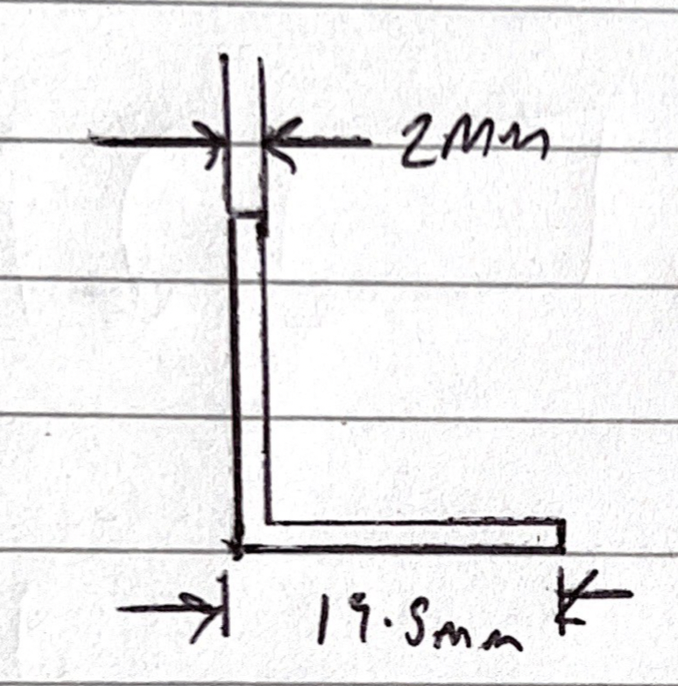
\includegraphics[height=14pc]{alu_angle.png}}
                        \end{minipage}%
                        \begin{minipage}[b]{14pc}{}
                            \centering
                            \subfloat[][Stress calculations]{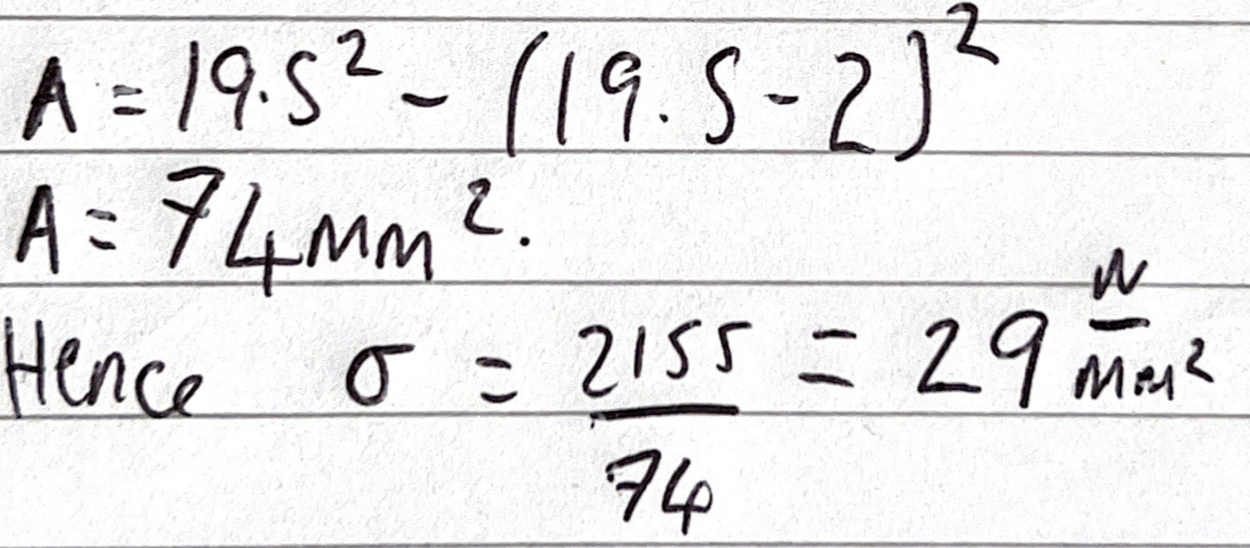
\includegraphics[width=14pc]{stress_calc.png}}
                        \end{minipage}\par\medskip
                        \caption{Handwritten diagram of the trusses and stress calculations for compression member}
                        \end{center}
                    \end{figure}
                    Hence at working load the stress is exactly 1/2 of failure, and therefore at ultimate load the stress would be roughly 60 N / mm$^2$ so that would be suitable to fail within
                    $\pm$5\% of failure load. At ultimate the stress would be 4310/74 which is 58 N / mm$^2$. This meant that bracing was needed at L/2 for horizontal and vertical. For the bracing
                    the smallest member was chosen as they don't theoretically carry any force, so the smallest angle should suffice.
                \subsubsection{Tension member}
                    The force in each tension member at ultimate load is 4.52 kN. Using the largest beams and assuming a stress calculated prior of 58 N / mm$^2$ - the failure
                    stress of 6068 is around 250 N / mm$^2$, so there would be no issues in the tension member. We used the larger member in order to allow enough space for rivets to be
                    placed without edge effects.
                \subsubsection{Rivets}
                    Assuming that the maximum force carried by each member is roughly 4.5 kN - and that each rivet was individually able to carry a shear stress of around 1.3 kN,
                    4 rivets should allow for the transfer of 5.2 kN (assuming linearity upon adding more rivets sensibly spaced), so that is what was chosen as it was above the
                    ultimate load by a substancial amount. Rivets were spaced centre-centre by a dimension of 5mm in order to reduce effects caused by placing them too close together. 
                \subsubsection{End-plate}
                    A plate of 2mm thickness was chosen in order to ensure it did not fail prior to the buckling failure method previously described. It was the strongest available
                    and in the sake of keeping simplicity, it was chosen to make some aspects overengineered in order to ensure the calculated failure method was the actual rather than
                    trying to introduce many failure methods and possibly having them co-join to form a weaker structure due to an oversight. 
                \subsubsection{Joint to base-plate}
                    It is important that the compression member is snug against the baseplate so that force can be easily transferred to the baseplate from the angle and not solely from the rivets.
                    Failure to do this would result in the rivets possibly shearing early.
            \subsection{Drawings of final design}
            \begin{figure}[H]
                \begin{center}
                \captionsetup{labelfont=bf}
                \captionsetup{justification=centering}
                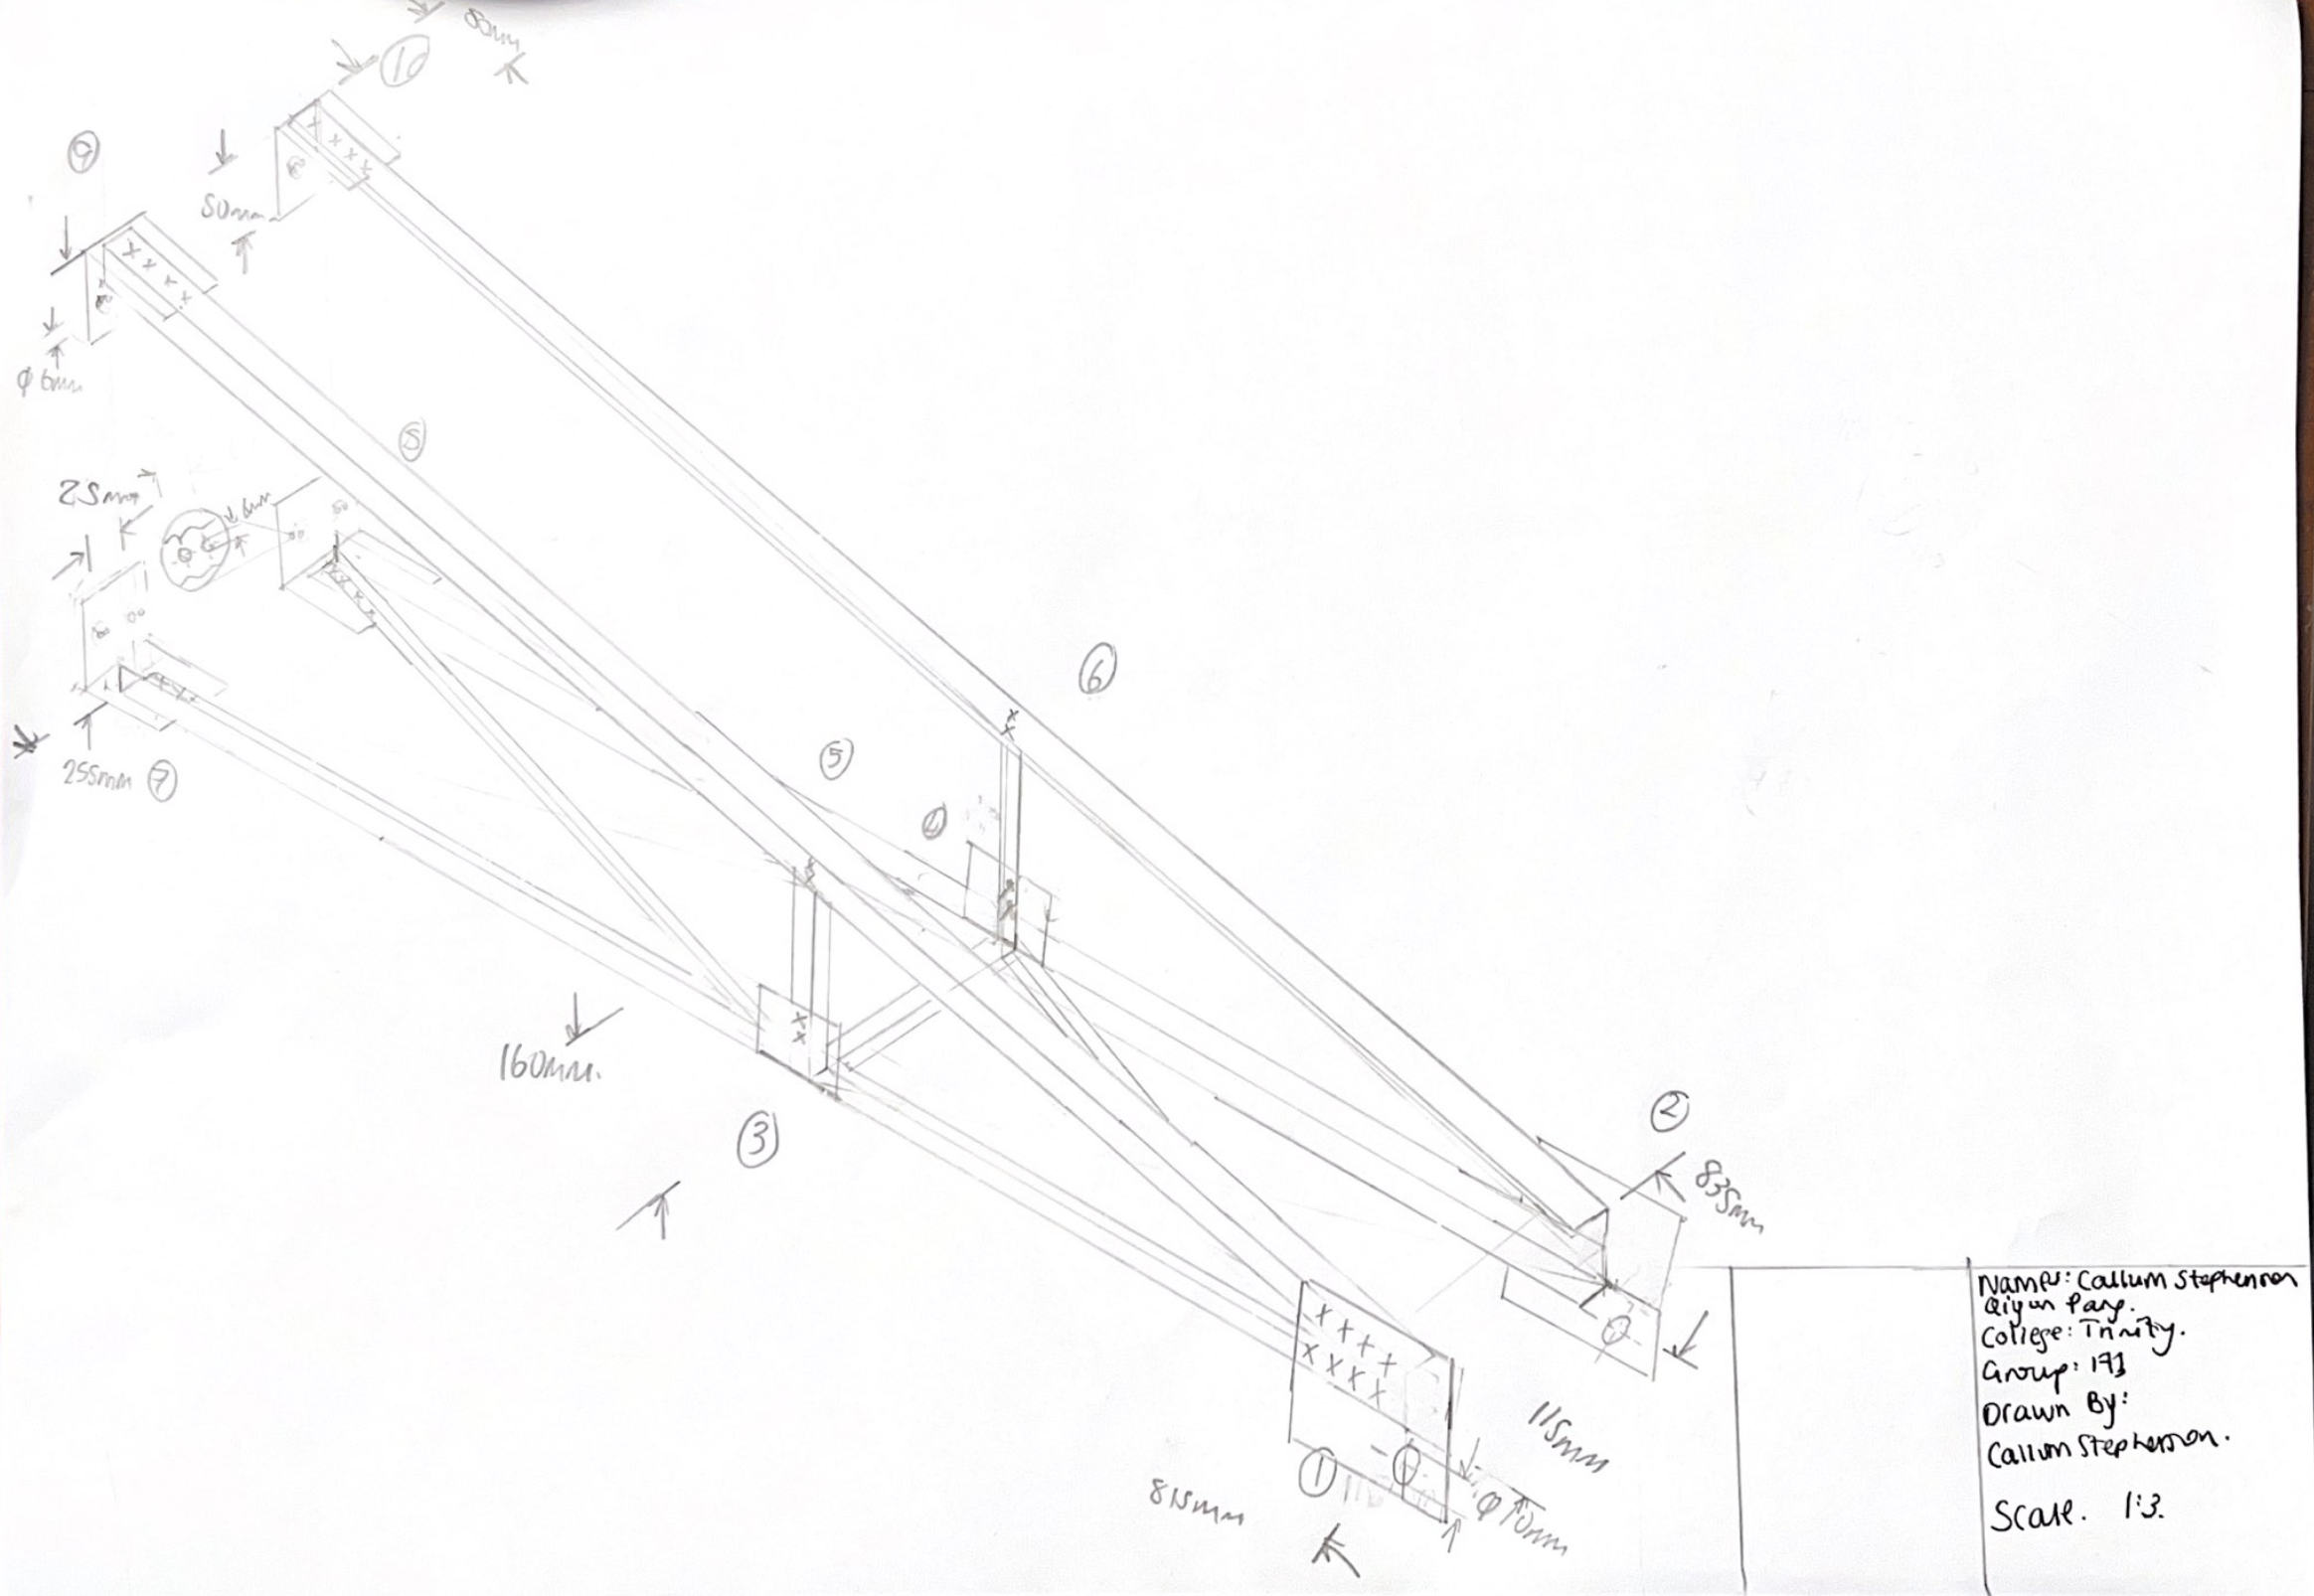
\includegraphics[height=17pc]{drawing_iso.png}
                \caption{Figure showing the isometric view of the final design}
                \end{center}
            \end{figure}
            \begin{figure}[H]
                \begin{center}
                \captionsetup{labelfont=bf}
                \captionsetup{justification=centering}
                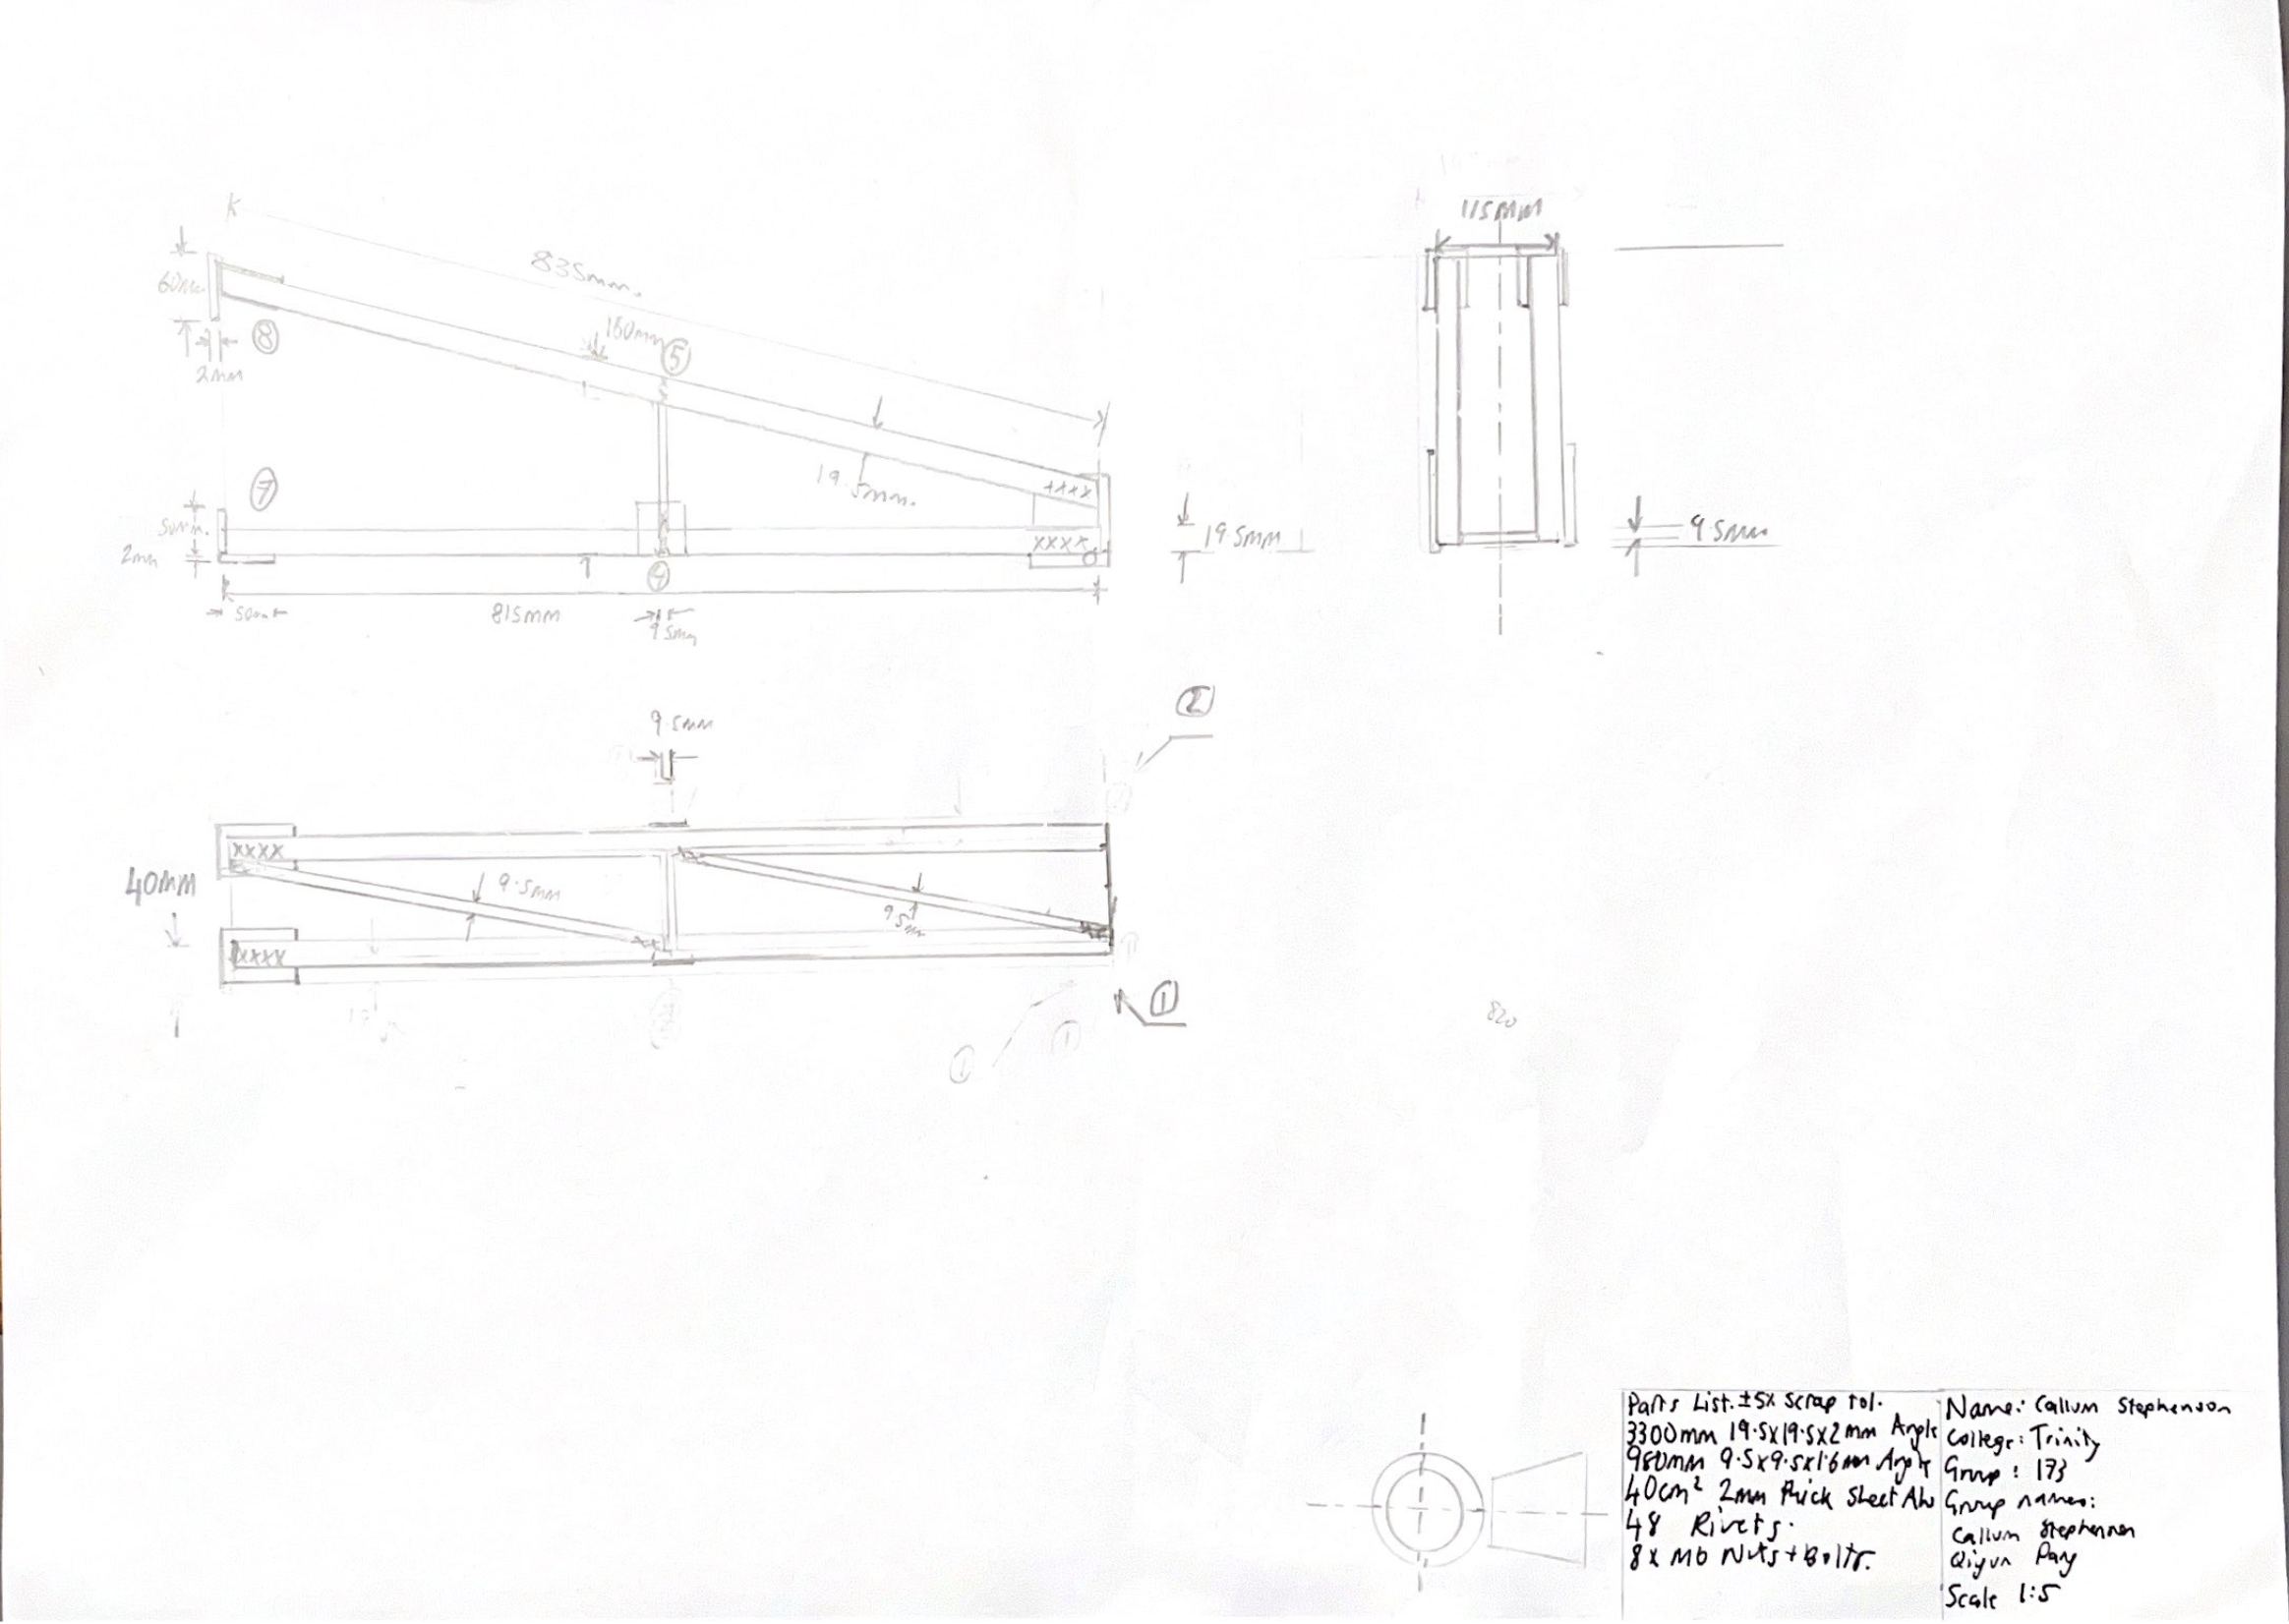
\includegraphics[height=17pc]{drawing_ortho.png}
                \caption{Figure showing the principle orthographic views of the final design}
                \end{center}
            \end{figure}
    \section{Deviation and costing sheet}
    During the design process there was not much deviation from the planned design. Rivets were chosen to be spaced 1cm apart instead of .5cm as spacing allowed. The structure had some
    manufacturing defects as the tension members were not properly butted up against the baseplate. We had a small error in drawings that the structure would not be centred, 
    but this was addressed and everything ran central with how it should be as to not introduce any rotation into the structure. The finished structure ended up weighing 1.02 Kg,
    which was near middle of all the structures. 
    \begin{figure}[H]
        \begin{center}
        \captionsetup{labelfont=bf}
        \captionsetup{justification=centering}
        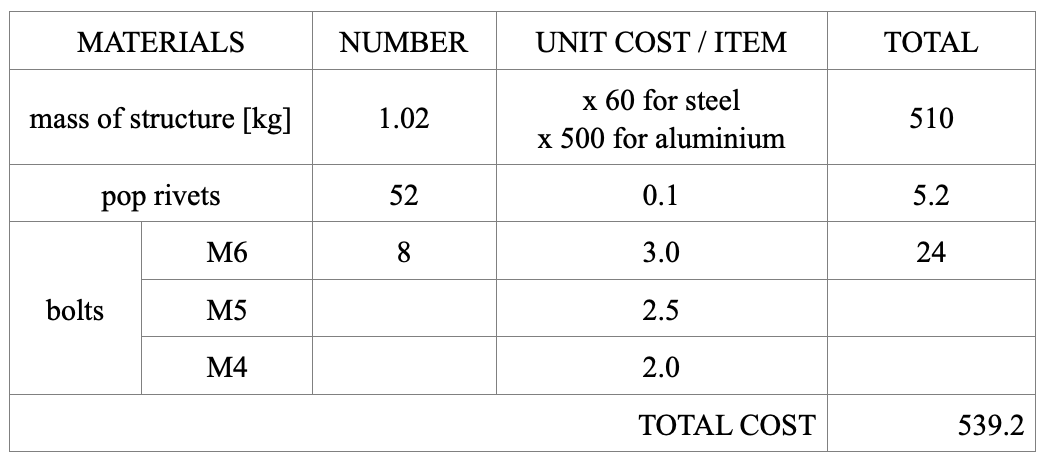
\includegraphics[height=17pc]{costing_sheet.png}
        \caption{Figure showing the costing sheet of the final design}
        \end{center}
    \end{figure}
    \section{Test results}
        The structure won out of all the structures within the cohort. It was the only structure to pass the three requirements - but was still not absurdly heavy. The structure
        was able to withstand 2.77 kN before failure, which is around what was expected. The expected failure mechanism was buckling as predicted in the design process, and it turned out
        that the actual mode of failure was buckling in mode A as calculated. Choosing to focus on one aspect to have fail instead of trying to encorporate multiple failure mechanisms seemed
        to be what differed between our design and the rest of the cohort, as sometimes their failure mechanisms worked against one another to create an overall weaker structure. Most common
        failure was weakness within the structure itself which allowed bending of the structure downwards - meaning the structure was unable to take more load. The second most was rivet shearing,
        where some groups had not taken into account the shear force at ultimate load and therefore their structures would prematurely break due to sheer. The runner up was an amazing
        isoscles design which very nearly passed the third test, but fell around 100 N shy. It was also relatively heavy (the heaviest infact) due to the necessity of multiple angles co-joined per side.
    \section{Modification}
        There are a few changes which could be implemented in order to reduce the weight of the structure whilst still maintaining the structural integrity up until the ultimate load.
        One of which is reduction of the size of the tension member, as it does not need to withstand as much stress as it is built for - but a bigger size was chosen to try to
        reduce visible deformation. A suitable swap would be for the 12.5 x 12.5 x 1.6 mm angle, which would have stresses of roughly 120 N / mm$^2$ - still much lower than 6068 yield stress of
        250 N / mm$^2$. This would've reduced weight quite a bit without the sacrifice of much structural integrity. Another change could be to reduce the end-plate area such that
        it doesn't have extra material on the top - again reducing weight.
    \section{Conclusion}
        The structure outlined within this report was relatively successful and passed the three tests successfully. This is in part due to the overengineering of some aspects whilst
        having a simple known failure mechanism at the ultimate load. As our design was relatively simple, the manufacturing process was relatively short which is another aspect to consider
        when having to manufacture a structure. Simplicity is sometimes best, as complex designs can introduce manufacturing defects beyond the designers' control which ultimately cause failure. \\ \\


        By keeping to a simple design, we were able to predict the actual mode of failure relatively accurately as well as the load at which failure would occur. Done again, it would be nice to
        try to minimise the weight with some of the easy weight saving measures - but also through use of software in order to calculate exactly what would happen as some groups
        had strange phenomena within their failure mechanism which would likely be explained by load calculation software.

        Overall, the design and testing of our structure was successful and we were pleased with the outcome and that our calculations proved accurate.
\end{document}